\documentclass[a4j]{jarticle}

\title{機能仕様書}
\date{\today}
\usepackage[dvips]{graphicx}

\begin{document}

\maketitle

\tableofcontents

\newpage

\section{概要}
本アプリケーションはユーザが今までに作成したCプログラムファイルの管理を行うためのものである。本アプリケーションを用いることで、作成したCソースファイル、実行ファイル、MAkefileなどのプログラム関連のファイルや、図形ファイル、Texファイルなどレポートに関するファイルまで管理することができる。アプリケーションの機能として、以下のものが挙げられる。\\
・任意のファイルの保存、読み込み\\
・複数のファイルから構成されるプログラム\footnote{複数のファイルから構成されるプログラムとは、複数のCソースファイル(メインルーチン、ソート関数部、入出力機能など)からなるプログラムを指す。}の登録\\
・新規データの追加、既存データの削除や参照\\
・任意のデータ、任意の項目に対しての修正\\
・新たな分類項目の追加、削除\\
・ユーザが任意に設定したタイトル名、副タイトル名、作成日付、ファイルのパス名、分類の項目によるファイルの検索、昇順ソート、降順ソート\\

本アプリケーションの利便性として、ファイルの管理が容易になることが挙げられる。ユーザは端末エミュレータにUNIXコマンドを打ち込むことなくファイルの管理ができる。

\newpage

\section{使用方法}
本アプリケーションはユーザが過去に作成したCプログラムファイルやそれに関連するファイルを参照したいときや、ファイルの整理をするときに利用されると想定される。また、すべての機能はUNIXコマンドを入力することなく使用することができるので、ユーザは新たなファイルの作成や削除なども容易に行うことができる。大まかな使用手順を次に示す。
\begin{enumerate}

\subsection{使用手順}

\item 機能一覧が表示される
\item ユーザは使用したい機能を選択する(機能名の隣に表示される番号で選択)
\begin{enumerate}


\item 新規プログラムの登録
\begin{enumerate}
\item 登録したいファイルのデータを入力(タイトル名、副タイトル名、作成日付、ファイルのパス名、分類項目)\footnote{複数のファイルから構成されるプログラムを登録する場合はタイトルにプログラム名(演習課題1など)、副タイトルにファイルの機能(メインルーチンなど)を入力}
\item 登録後のファイル一覧を表示
\end{enumerate}


\item 既存データの参照
\begin{enumerate}
\item 参照したいファイルを探すためのキーとなるデータを入力(タイトル名、副タイトル名、作成日付、ファイルのパス名、分類項目の中から選択して入力)
\item 入力されたキーに一致したファイル一覧を表示
\end{enumerate}

\item 既存データの削除
\begin{enumerate}
\item 削除したいファイルを探すためのキーとなるデータを入力(タイトル名、副タイトル名、作成日付、ファイルのパス名、分類項目の全てを入力)
\item 入力されたキーに一致したファイルを表示
\item 本当に削除するかを選択
\item 指定したファイル削除後のファイル一覧を表示
\end{enumerate}

\item 任意のファイル、任意の項目に対しての修正
\begin{enumerate}
\item 修正したいファイルルを探すためのキーとなるデータを入力(タイトル名、副タイトル名、作成日付、ファイルのパス名、分類項目の全てを入力)
\item 入力されたキーに一致したファイル一覧を表示
\item 修正する項目、修正後のデータを入力
\item 修正後のファイルのデータを表示
\end{enumerate}

\item 新たな分類項目の追加
\begin{enumerate}
\item 追加したい分類項目名を入力
\item 追加後の分類項目一覧を表示
\end{enumerate}

\item 既存の分類項目の削除
\begin{enumerate}
\item 削除したい分類項目名を入力
\item 入力された分類項目に一致した分類項目を表示した後、本当に削除するか選択
\item 削除後の分類項目一覧を表示
\end{enumerate}

\item ファイル一覧のソート
\begin{enumerate}
\item ソート方法を選択(選択肢の中から選択)
\item ソート後のファイル一覧を表示
\end{enumerate}
\end{enumerate}
\end{enumerate}

\subsection{使用手順概念図}
\resizebox{\textwidth}{!}{\rotatebox{270}{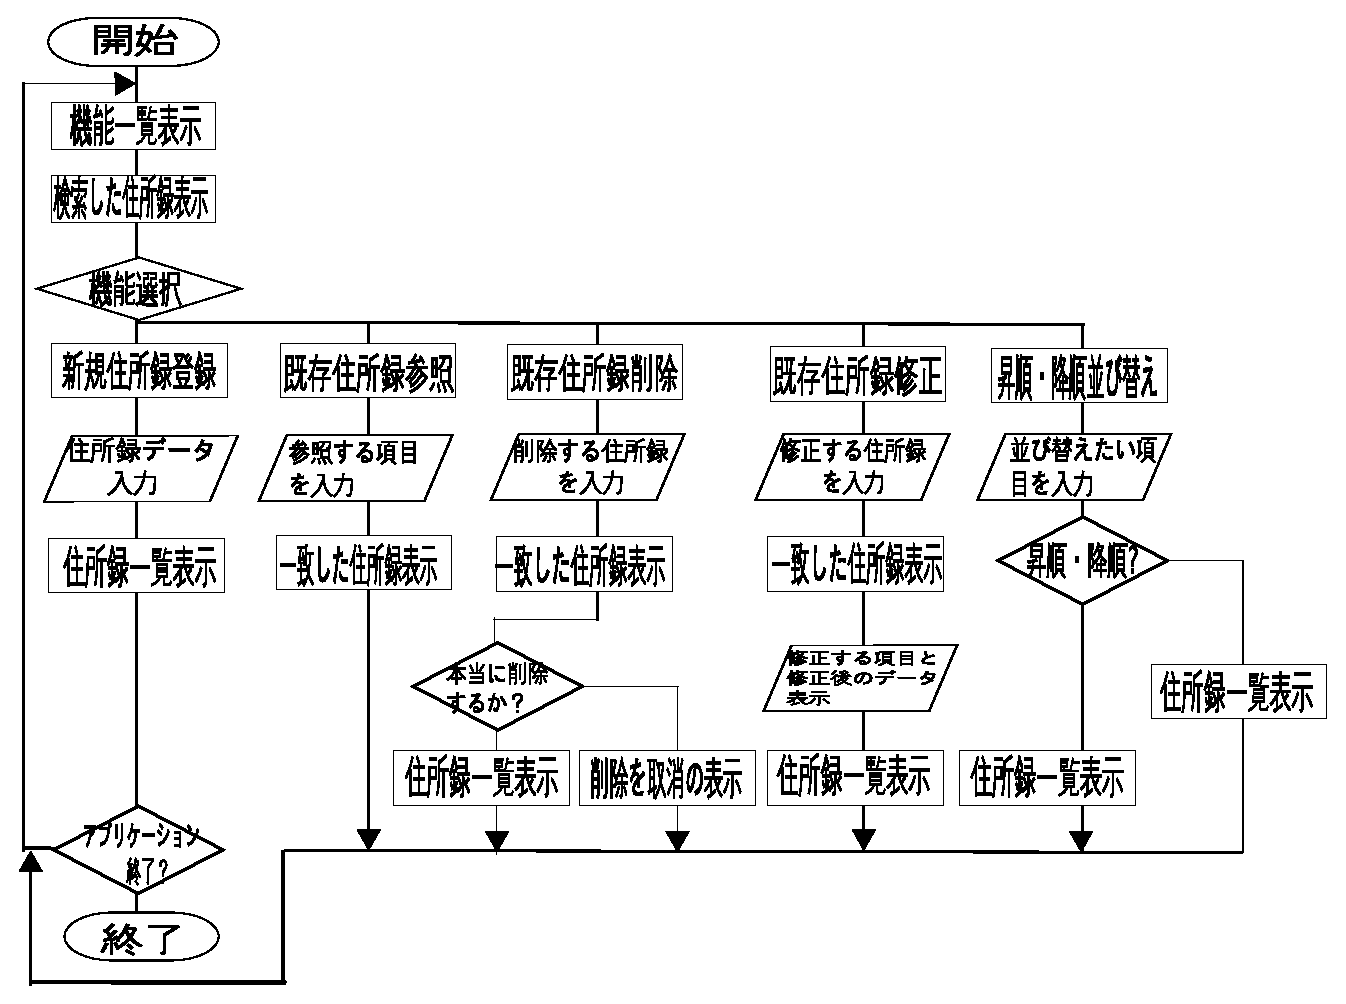
\includegraphics{flowchart1.eps}}}

\newpage

\section{画面イメージ}
本アプリケーションを使用する際の画面イメージを機能毎に示す。各画面イメージは選択肢のうち1つを選択した場合のみを例として載せている。
\begin{figure}[h]
\subsection{機能選択画面}
\includegraphics{template.eps}
\caption{機能選択画面}
\end{figure}

\begin{figure}[h]
\subsection{新規データの登録}
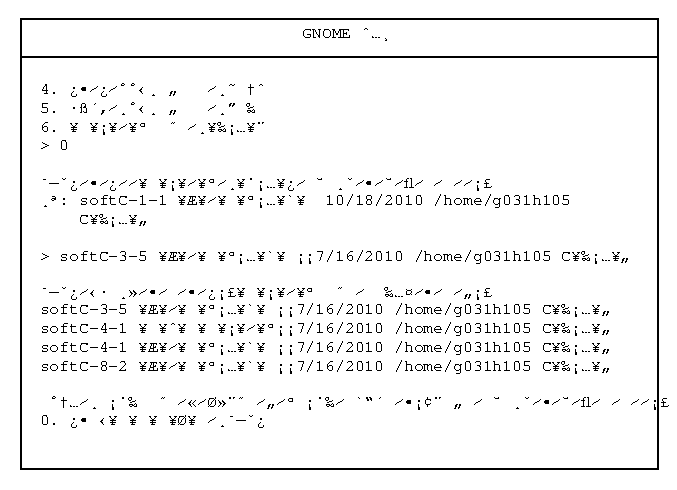
\includegraphics{new_program.eps}
\caption{新規データの登録}
\end{figure}

\begin{figure}[h]
\subsection{既存データの参照}
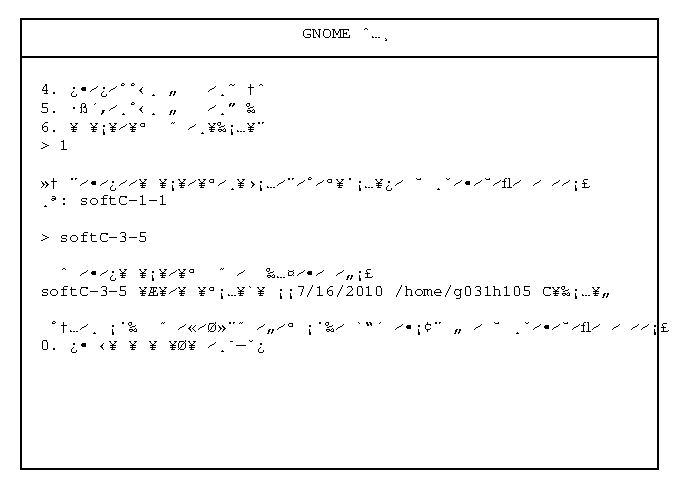
\includegraphics{data_view.eps}
\caption{既存データの参照}
\end{figure}

\begin{figure}[h]
\subsection{既存データの削除}
\includegraphics{data_del.eps}
\caption{既存データの削除}
\end{figure}

\begin{figure}[h]
\subsection{任意のファイル、任意の項目に対しての修正}
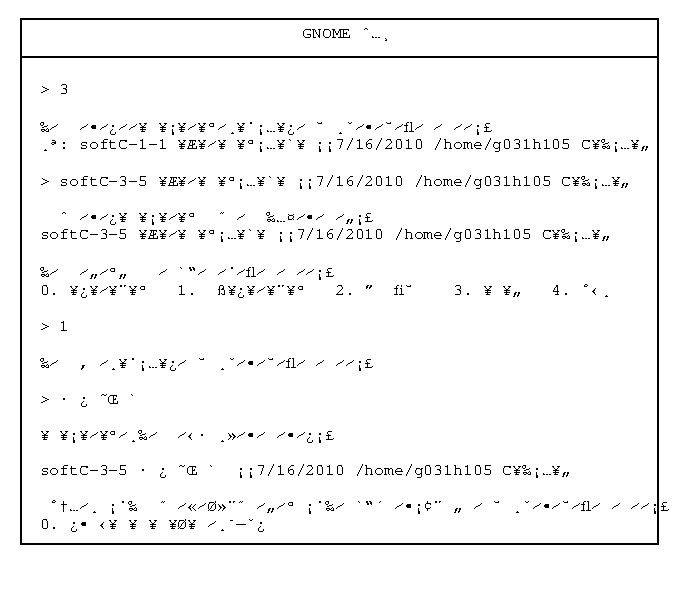
\includegraphics{data_remake.eps}
\caption{任意のファイル、任意の項目に対しての修正}
\end{figure}

\begin{figure}[h]
\subsection{新たな分類項目の追加}
\includegraphics{add_category.eps}
\caption{新たな分類項目の追加}
\end{figure}

\begin{figure}[h]
\subsection{既存の分類項目の削除}
\includegraphics{del_category.eps}
\caption{既存の分類項目のさ駆除}
\end{figure}

\begin{figure}[htb]
\subsection{ファイル一覧のソート}
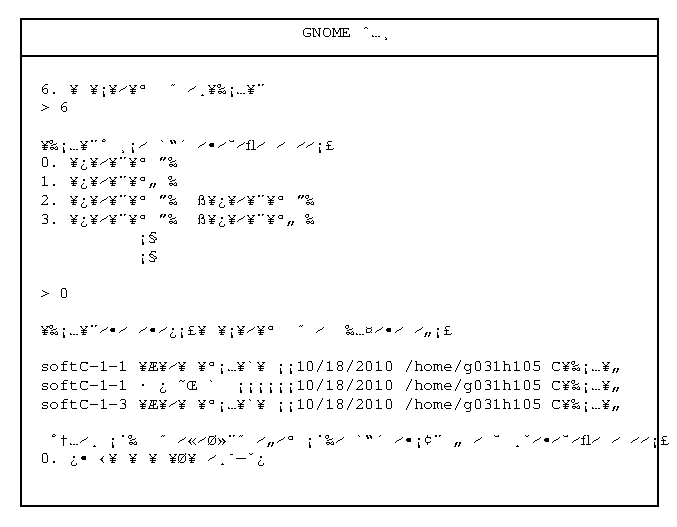
\includegraphics{data_sort.eps}
\caption{ファイル一覧のソート}
\end{figure}

\end{document} 
